\documentclass[tikz, border=10pt]{standalone}
\usetikzlibrary{calc, positioning, decorations.pathreplacing, arrows.meta}

% Style definitions
\tikzset{
  % Grid cell style
  cell/.style={rectangle, draw=gray!50, thick, minimum size=1.2cm, inner sep=0pt, font=\large},
  % Highlight styles
  rowhl/.style={fill=blue!15, draw=blue!60, thick},
  colhl/.style={fill=orange!20, draw=orange!70, thick},
  reshl/.style={fill=purple!15, draw=purple!60, thick},
  % Labels
  matlabel/.style={font=\large\bfseries},
  oplabel/.style={font=\Huge},
}

\begin{document}
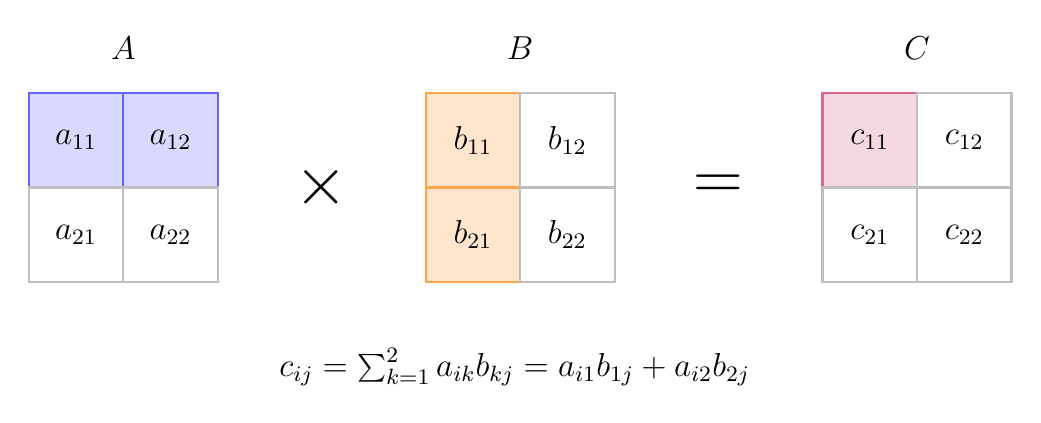
\begin{tikzpicture}[x=1.2cm, y=1.2cm]
  \def\n{2} % Matrix dimension (2x2)

  % --- MATRIX A ---
  \begin{scope}[shift={(0,0)}]
    \node[matlabel, above=0.3cm] at (\n/2, \n) {$A$};
    \node[cell, rowhl] (A-1-1) at (0.5, 1.5) {$a_{11}$};
    \node[cell, rowhl] (A-1-2) at (1.5, 1.5) {$a_{12}$};
    \node[cell]       (A-2-1) at (0.5, 0.5) {$a_{21}$};
    \node[cell]       (A-2-2) at (1.5, 0.5) {$a_{22}$};
  \end{scope}

  % Multiplication operator
  \node[oplabel] at (3.1, \n/2) {$\times$};

  % --- MATRIX B ---
  \begin{scope}[shift={(4.2,0)}]
    \node[matlabel, above=0.3cm] at (\n/2, \n) {$B$};
    \node[cell, colhl] (B-1-1) at (0.5, 1.5) {$b_{11}$};
    \node[cell]       (B-1-2) at (1.5, 1.5) {$b_{12}$};
    \node[cell, colhl] (B-2-1) at (0.5, 0.5) {$b_{21}$};
    \node[cell]       (B-2-2) at (1.5, 0.5) {$b_{22}$};

  \end{scope}

  % Equals sign
  \node[oplabel] at (7.3, \n/2) {$=$};

  % --- MATRIX C ---
  \begin{scope}[shift={(8.4,0)}]
    \node[matlabel, above=0.3cm] at (\n/2, \n) {$C$};
    \node[cell, reshl] (C-1-1) at (0.5, 1.5) {$c_{11}$};
    \node[cell]       (C-1-2) at (1.5, 1.5) {$c_{12}$};
    \node[cell]       (C-2-1) at (0.5, 0.5) {$c_{21}$};
    \node[cell]       (C-2-2) at (1.5, 0.5) {$c_{22}$};

  \end{scope}

  % --- Dot Product Formula ---
  \node[align=center, font=\large] at (5.2, -0.9) {
    $c_{ij} = \sum_{k=1}^{2} a_{ik} b_{kj} = a_{i1}b_{1j} + a_{i2}b_{2j}$
  };

\end{tikzpicture}
\end{document}
